\documentclass[10pt,letterpaper]{article}
\usepackage{fullpage}
\usepackage{xcolor}
\usepackage[top=1in, bottom=1in, left=1in, right=1in]{geometry}
\usepackage{graphicx}
\usepackage{wrapfig}
\usepackage{hyperref}

\newcommand{\todo}[1]{\textcolor{red}{TODO:\ #1}}

\title{ECE6745 Project Proposal}
\author{Matthew Hofmann}
\date{\today}

\begin{document}

\maketitle

\section{Motivation}\label{sec:motivation}

As the trends of transistor scaling come to a close, the QoR (quality of
results) of EDA tools will become more of a bottleneck in the hardware design
process. Given new developments in compiler technology and automated reasoning
tools, it is possible to better study the suboptimality of the EDA tool stack.
Several of the heuristics used in core EDA algorithms were invented decades
ago, and increases in compute capacity in the modern era afford us a more
formal and exploratory approach to optimizing digital logic. In this project, I
hope to use the automated reasoning capabilities of equivalence graphs
(e-graphs) to more precisely explore optimal designs points in the PPA (power,
performance, area) trade-off space. I predict that e-graph driven compilers can
better span the wide gap between SAT-based, exact synthesis and fully heuristic
algorithms.

\section{Project Proposal}\label{sec:intro}

In the last 6 months, I have started a project that uses e-graphs to
superoptimize FPGA netlists. In that amount of time, I have some pretty
compelling results. Across 96 academic benchmarks, my tool, called E-Pack,
reduces FPGA LUT count by 12\% on average over vendor tools. My current results
are for FPGAs, but I am optimistic that my compiler infrastructure can be
re-used for ASIC design as a course project. In total, I have three experiments
planned ordered from most conservative to furthest reach goal:

\begin{enumerate}
    \item Equivalence Checking and Program Fuzzing:

          \hspace{2em}\begin{minipage}{0.8\linewidth}
              (1) I will adapt my e-graph+Verilog tool to perform RTL equivalence checking and evaluate it against other tools (SAT solvers, verification tools, Jasper).

              (2) I will also use my tool to generate random correct or incorrect changes to netlists to test the stability in quality of results through place and route.

              This is my least ambitious plan and is mostly a backup to the next two.
          \end{minipage}

    \item Standard Cell Library Development:

          \hspace{2em}\begin{minipage}{0.8\linewidth}
              I will develop a methodology to measure the incremental advantage of adding more standard cells to a library.
              I will seek to quantify how much area or delay can be saved by introducing a new cell type into a library. This will of course require many benchmarks and re-synthesis of netlists.
              E-graphs afford the adaptability to rapidly re-synthesizing to different cell libraries.
          \end{minipage}

    \item More Exact Synthesis:

          \hspace{2em}\begin{minipage}{0.8\linewidth}
              I will provide a post-synthesis optimization tool that will improve upon the implementation results of Synopsys Design Compiler.
              E-graphs can certainly explore improved circuit topologies, but the real challenge will be creating an extraction algorithm that can improve upon the starting point given by Synopsys DC.
              Optimizing for delay may be more feasible than optimizing for area.
          \end{minipage}
\end{enumerate}

All of these experiments are relatively low cost to start, because I have a lot
of compiler infrastructure already built up. For instance, I have a custom,
bare-bones SystemVerilog frontend. After some initial experiments, I plan to
choose the one topic which shows the most promise. In the following sections, I
will give the background needed to understand equivalence graphs for compiler
development as well as some more detailed planning.

\section{Background}\label{sec:background}

Equivalence graphs, most commonly referred to as \textit{e-graphs}, are an
automated reasoning tool built around a union-find data
structure~\cite{eggpaper}. An e-graph is essentially a directed graph with two
extra features: (1) nodes are grouped together into \textit{e-classes} and (2)
edges always start at a node and point to an e-class. As a consequence,
e-graphs can very compactly store a collection of equivalence relations. The
prototypical example for e-graphs involves the rewriting of arithmetic
expressions. For instance, one relation conveyed in Fig.~\ref{fig:egraph} is
that \texttt{a << 1} is equal to \texttt{a * 2}. To convey equality, the
anchoring nodes \texttt{<<} and \texttt{*} are grouped in the same e-class (the
dotted box). The children of the operators are the e-classes for \texttt{a},
\texttt{2}, and \texttt{1}. It is typical that constants and variables are leaf
nodes that live in an e-class alone. However, it is important to note that the
destination of edges is always an e-class and not a node. With this
illustration, it hopefully becomes clear why e-graphs are strong at equational
reasoning. The next section will explain how we can build an optimizing
compiler out of this design.

\begin{wrapfigure}{r}{0.47\textwidth}
    \centering
    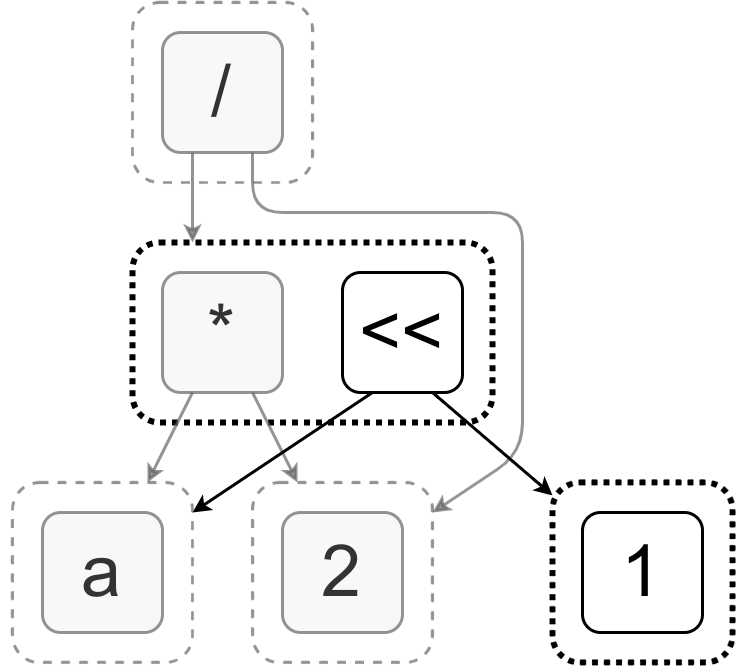
\includegraphics[width=0.44\textwidth]{img/egraph.png}
    \caption{An e-graph with 5 e-classes and 6 e-nodes.}\label{fig:egraph}
\end{wrapfigure}

E-graphs cannot reason on their own: one needs to define the notions of
equality unique to their problem domain. Continuing with the example of
computer arithmetic, we can declare arithmetic properties, like commutativity,
associativity, and distributivity, with \textit{rewrite rules}. For example,
the syntax \texttt{?a + ?b => ?b + ?a} would encode commutativity as a rewrite
rule. The left-hand side denotes a pattern to search for in the e-graph, and
the right side encodes the application of the rule. If the right-hand side of a
rule already exists in the e-graph, its e-class will be merged with the e-class
matched from the left-hand side. Otherwise, the application is inserted as a
new node in the e-class. It is important that rewrite rules are atomic. If a
rule can be broken down into multiple smaller rules, they should. This way you
can better rationalize what types of expression topologies are reachable by
your e-graph.

When using e-graphs to drive a compiler, you place your starting
expression/circuit in an empty e-graph, and each node starts alone in its
e-class. Then, you use the collection of rewrite rules to grow and build the
e-graph with alternative representations. When rewrite rules no longer
introduce new information into the graph, we say we have reach \textit{equality
    saturation}. In many cases, such as Boolean circuits, it is not possible to
fully saturated the e-graph. Instead, a time limit or size limit is reached.
Once the e-graph is built, all that is left is to extract the best rewriting of
the expression. This of course is the NP-hard part. There are several research
projects on e-graph extraction~\cite{smoothe,sparsextract}, but they are beyond
the scope of this course project. However, previous work on FPGA technology
mapping has demonstrated that fast, greedy extraction algorithms can be used
and still find area and circuit depth improvements.

In the end, e-graph driven compilers are less heuristic than conventional
compiler architectures, because they transform terms non-destructively. Typical
optimizing compilers are broken down into a pass pipeline, and the quality of
results is sensitive to the ordering of these optimization passes. Optimizing
compilers built around passes will never be able to generalize to all programs,
but in practice the results are adequate for software. In the hardware domain,
the rules of economies of scale apply and Moore's law scaling is over. Finding
an optimal design point within tight design constraints is paramount. As a
solution, e-graphs are a more formal and more optimal approach to problems in
electronic design automation. Previous work~\cite{esyn} has demonstrated the
usefulness of e-graphs for logic synthesis. Moreover, I hope to submit my own
e-graph work to ICCAD which shows 12\% area savings over vendor tools on FPGA
applications without increasing circuit depth.

\section{Experiment Design}\label{sec:experiments}

Each of the three ideas for experimentation will require a decently large
collection of Verilog benchmarks. In total, I have a collection of 96 RTL
benchmarks combined from three academic sources: ISCAS'85, LGSYNTH'91, and
EPFL\footnote{\href{https://github.com/matth2k/synth-benchmarks}{https://github.com/matth2k/synth-benchmarks}}.
They are mostly combinational benchmarks, but sequential logic can also be
tested. In general, I will consider Synopsys Design Compiler as the baseline
synthesis tool.

\subsection{Equivalence Checking and Program Fuzzing}
Yosys will act as the baseline verification tool. Depending on the other tools
we have licenses for (Jasper?), I can also compare their verification abilities
as well. One hypothesis to test is if e-graphs can more quickly or more
robustly give conclusions to RTL equivalence checking problems. In addition, I
want to test the stability of QoR of place and route tools given small changes
in logic synthesis behavior. In other words, can we precisely observe the
interactions between synthesis and place and route? Can we use formal tools to
prevent negative interactions between these two phases of design? These
verification and fuzzing tasks will require writing the equivalance checking
and fuzzing tools, but this will largely reuse my existing e-graph rewriting
framework. Then, we will evaluate the verification tools and synthesis tools on
fuzzed versions of the Verilog benchmark suite. Of course, we can introduce
errors as part of the fuzzing.

\subsection{Standard Cell Library Development}

This experiment plans to develop a methodology for measuring the incremental
improvement of adding more cell types to a standard cell library. This means
that the baseline will be some restricted cell library, and the results will be
the incremental improvements in post-synthesis area and timing as new cell
types are added. The measurements will of course depend on the test cases, so I
will have to ensure that my benchmark suite is general enough. The hypothesis
being tested is that e-graphs plus extraction formulate a more adaptable
compiler architecture without sacrifices in quality. It will also provide
insight into the trade-off space of standard cell library design.

\subsection{More Exact Synthesis}
In this experiment, I will develop logic rewriting systems and extraction
techniques that can achieve better results than Synopsys Design Compiler. In
the case of FPGA technology mapping, I already have results that show 12\% area
savings over the vendor tools without degrading timing. Moreover, I already
have a robust Boolean logic rewriting system that can be extended to standard
cell design. However, the potential pitfalls come with extraction technique.
While greedy extraction shows promise for FPGA applications, I have gut
feelings that the same extraction algorithm will not work as well for ASIC
design. ASIC cell mapping appears less like a graph covering algorithm, because
most of the cells have fanin of 1-3. FPGAs, on the other hand, have 6 input
lookup tables. Nonethless, I could be underestimating the flexibility of
standard cell design. Perhaps basic greedy extraction algorithms would still
work for synthesizing to standard cells. Moreover, I anticipate that new
e-graph extraction algorithms will improve its circuit synthesis abilities.
Although, developing new extraction algorithms is more pure compilers research
than EDA research.

\nocite{*}
\bibliographystyle{plain-annote}
\bibliography{references}

\end{document}